\documentclass{article}
\usepackage[utf8x]{inputenc}
\usepackage{ucs}
\usepackage{amsmath} 
\usepackage{amsfonts}
\usepackage{marvosym}
\usepackage{wasysym}
\usepackage{upgreek}
\usepackage[english,russian]{babel}
\usepackage{graphicx}
\usepackage{float}
\usepackage{textcomp}
\usepackage{hyperref}
\usepackage{geometry}
  \geometry{left=2cm}
  \geometry{right=1.5cm}
  \geometry{top=1cm}
  \geometry{bottom=2cm}
\usepackage{tikz}
\usepackage{ccaption}
\usepackage{multicol}

\hypersetup{
   colorlinks=true,
   citecolor=blue,
   linkcolor=black,
   urlcolor=blue
}

\usepackage{listings}
%\setlength{\columnsep}{1.5cm}
%\setlength{\columnseprule}{0.2pt}

\usepackage[absolute]{textpos}

\usepackage{colortbl,graphicx,tikz}
\definecolor{X}{rgb}{.5,.5,.5}


\begin{document}
\pagenumbering{gobble}
\lstset{
  language=C,                % choose the language of the code
  basicstyle=\linespread{1.1}\ttfamily,
  columns=fixed,
  fontadjust=true,
  basewidth=0.5em,
  keywordstyle=\color{blue}\bfseries,
  commentstyle=\color{gray},
  stringstyle=\ttfamily\color{orange!50!black},
  showstringspaces=false,
  numbersep=5pt,
  numberstyle=\tiny\color{black},
  numberfirstline=true,
  stepnumber=1,                   % the step between two line-numbers.        
  numbersep=10pt,                  % how far the line-numbers are from the code
  backgroundcolor=\color{white},  % choose the background color. You must add \usepackage{color}
  showstringspaces=false,         % underline spaces within strings
  captionpos=b,                   % sets the caption-position to bottom
  breaklines=true,                % sets automatic line breaking
  breakatwhitespace=true,         % sets if automatic breaks should only happen at whitespace
  xleftmargin=.2in,
  extendedchars=\true,
  keepspaces = true,
}
\lstset{literate=%
   *{0}{{{\color{red!20!violet}0}}}1
    {1}{{{\color{red!20!violet}1}}}1
    {2}{{{\color{red!20!violet}2}}}1
    {3}{{{\color{red!20!violet}3}}}1
    {4}{{{\color{red!20!violet}4}}}1
    {5}{{{\color{red!20!violet}5}}}1
    {6}{{{\color{red!20!violet}6}}}1
    {7}{{{\color{red!20!violet}7}}}1
    {8}{{{\color{red!20!violet}8}}}1
    {9}{{{\color{red!20!violet}9}}}1
}
\newpage

\title{Семинар \#14: Сегмент памяти текст. Классные задания.\vspace{-5ex}}\date{}\maketitle
\section*{Часть 1: Сегмент памяти Текст. Указатели на функцию.}

\subsection*{Сегмент памяти \texttt{Text}}
\begin{itemize}
\item В этом сегменте хранится машинный код программы (Код на языке C, сначала, переводится в код на языке Ассемблера, а потом в машинный код. Как это происходит смотрите ниже.).
\item Адрес функции - адрес первого байта инструкций в этом сегменте.
\end{itemize}


\subsection*{Указатели на функции}
Пример работы с указателем на функцию:
\begin{lstlisting}
#include <stdio.h>

void print(int a)
{
    printf("%d\n", a);
}
int main ()
{
    // Создадим указатель на функцию ( вместо названия функции - *p )
    void (*p)(int a) = print;
    
    // Теперь с p можно работать также как и с print
    p(123);
}
\end{lstlisting}
Подробней в файле \texttt{funcpointers/0funcpointer.c}.
\textbf{Задачи на указатели на функцию:}
\begin{itemize}
\item В файле \texttt{funcpointers/1foreach.c} лежит заготовка исходного кода. Вам нужно написать функцию\\ \texttt{void foreach(int* array, int size, int (*f)(int))}, которая будет принимать на вход массив размера \texttt{size} и применять к каждому элементу функцию \texttt{f}.

\item В файле \texttt{funcpointers/2foreach\_second\_argument.c} лежит заготовка исходного кода. Вам нужно написать функцию\\ \texttt{void foreach(int* array, int size, int (*f)(int, int), int b)}, которая будет принимать на вход массив размера \texttt{size} и применять к каждому элементу функцию \texttt{g(x) = f(x, b)}.
\end{itemize}


\subsection*{Стандартная функция qsort}

В библиотеке \texttt{stdlib.h} уже реализована функция \texttt{qsort}, которая сортирует произвольные элементы, используя быструю сортировку. Пример использования этой функции:
\begin{lstlisting}
#include <stdio.h>
#include <stdlib.h>

int cmp(const void* a, const void* b)
{
    // В этот компаратор передаются указатели на void,
    // Поэтому их нужно привести в нужный нам тип:
    int* pa = (int*)a;
    int* pb = (int*)b;
    return (*pa - *pb);
}

int main()
{
    int arr[] = {163, 624, 7345, 545, 41, 78, 5, 536, 962, 1579};
    qsort(arr, 10, sizeof(int), cmp);
    // qsort( массив, количество элементов, размер каждого элемента, компаратор )
    // Функция принимает на вход указатель на функцию cmp
   
    print_array(10, arr);
}
\end{lstlisting}
Функция-компаратор стандартной функции \texttt{qsort} отличается от той, что была написана нами для сортировки
городов и звёзд только тем, что она принимает на вход указатели типа \texttt{void*}. Это сделано для того, чтобы эта функция была более общей. С помощью неё можно отсортировать как массив чисел, так и массив указателей или массив любых структур. В функции \texttt{cmp} нужно привести указатель \texttt{void*} к указателю нужного типа.\\
\textbf{Задача на стандартную функцию \texttt{qsort}:}
\begin{itemize}
\item Перепишите сортировку звёзд с использованием функции \texttt{qsort}.
\end{itemize}



\newpage
\section*{Часть 2: Как код превращается в последовательность байт.}
\begin{center}
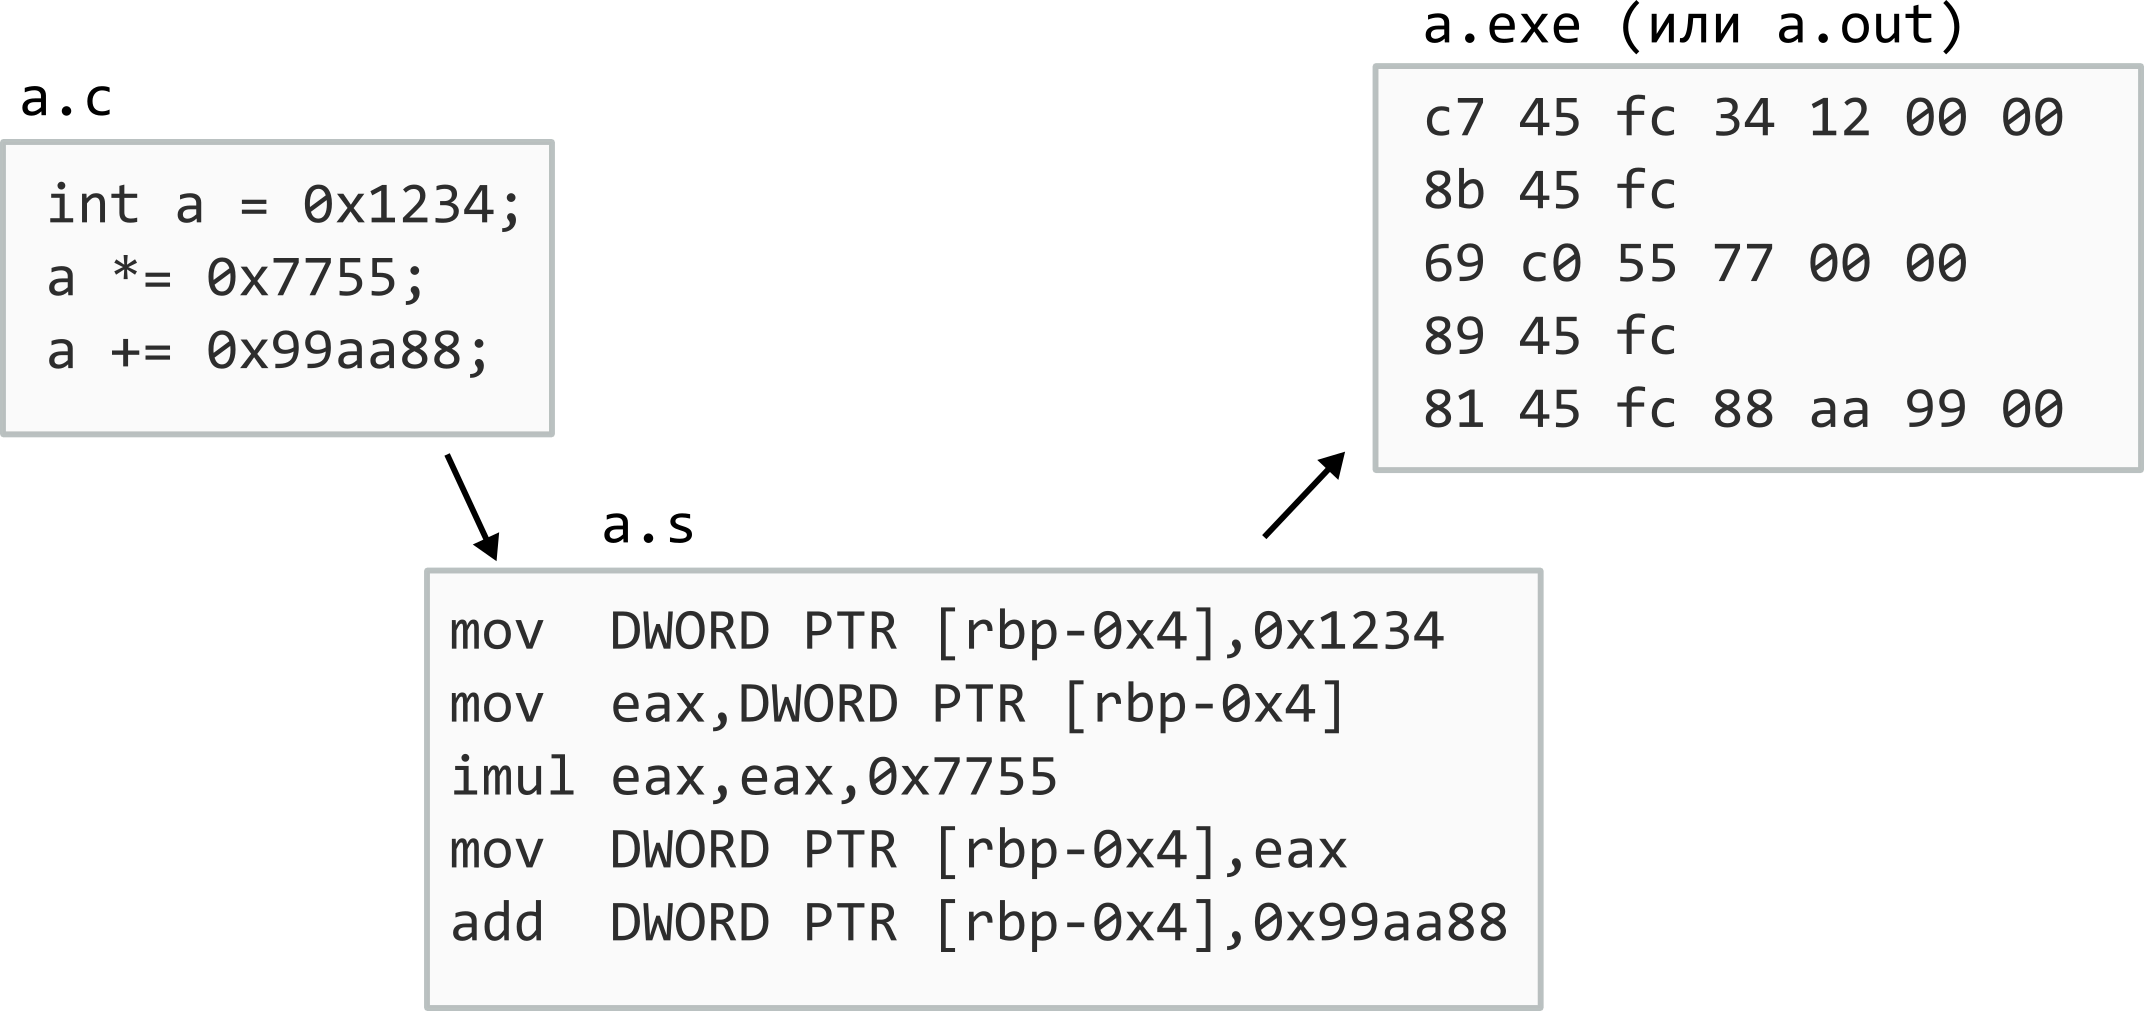
\includegraphics[scale=0.9]{../images/code_to_hex.png}
\end{center}
\subsubsection*{Из кода на C в код ассемблера:}
\begin{itemize}
\item Код на языке \texttt{C} (\texttt{a.c}) переводится в код на языке ассемблера (\texttt{a.s}). Эту операцию можно сделать командой
\begin{verbatim}
gcc -S -masm=intel ./a.c
\end{verbatim}
\item Регистры процессора -- это сверхбыстрая память, которая находится внутри процессора. Её размер очень мал(десятки байт), но процессор может доступиться к ней очень быстро (за 1 такт). В примере выше используются 2 регистра: \texttt{rbp} и \texttt{eax} (\texttt{eax} это часть регистра \texttt{rax}). 
\item Процессор может делать множество различных операций. Например, он может переместить некоторое количество байт из одного места в другое. Такие операции называются \texttt{mov}. Он может прибавить число (\texttt{add}) или умножить на целое (\texttt{imull}) и многое другое. \texttt{DWORD PTR} просто означает, что операция будет работать с 4-мя байтами.
\item В примере выше в регистре \texttt{rbp} содержится некоторый адрес. Квадратные скобочки означают разыменование. Поэтому строка
\begin{verbatim}
mov DWORD PTR [rbp-0x4],0x1234
\end{verbatim}
означает, что нужно положить число \texttt{0x1234} в 4 байта по адресу \texttt{rbp-0x4}
\item 
\begin{verbatim}
mov eax,DWORD PTR [rbp-0x4]
\end{verbatim}
означает, что нужно переместить 4 байта, которые хранятся по адресу \texttt{rbp-0x4} в регистр \texttt{eax}.
\item
\begin{verbatim}
imull eax,eax,0x7755
\end{verbatim}
означает, что нужно умножить содержимое \texttt{eax} на \texttt{0x7755} и сохранить результат в \texttt{eax}.
\item
\begin{verbatim}
mov  DWORD PTR [rbp-0x4],eax
\end{verbatim}
означает, что нужно переместить содержимое \texttt{eax} в память по адресу \texttt{rbp-0x4}.
\item
\begin{verbatim}
add  DWORD PTR [rbp-0x4],0x99aa88
\end{verbatim}
означает, что нужно добавить к числу по адресу \texttt{rbp-0x4} число \texttt{0x99aa88}.
\item В отличии от кода на языке \texttt{C}, код на языке ассемблера различаться на разных процессорах. Код с  вычислительной системы одной архитектуры скорей всего не будет работать на другой.
\end{itemize}
\subsubsection*{Из кода ассемблера в бинарный код (\texttt{.exe}):}
\begin{itemize}
\item Код на языке ассемблера (\texttt{a.s}) переводится в исполняемый файл. Эту операцию можно сделать командой \texttt{gcc a.s}
\item Каждая операция кодируется некоторым числом, называемым кодом операции (opcode).
\item Код операции \texttt{mov} на процессорах архитектуры \texttt{x86-64} может равняться \texttt{с7} или \texttt{8b} или \texttt{89} или некоторым другим  значениям(в зависимости от того куда и откуда мы копируем).
\item Например в строке:
\begin{verbatim}
c7 45 fc 34 12 00 00
\end{verbatim}
\begin{itemize}
\item \texttt{с7} означает, что это операция \texttt{mov} (присвоить число переменной в памяти)
\item \texttt{45} кодирует регистр \texttt{rbp}
\item \texttt{fc} кодирует смещение \texttt{-0x4}
\item \texttt{34 12 00 00} -- это 4-х байтовое число \texttt{0x1234} (порядок байт -- Little Endian)
\end{itemize}

\item
\begin{verbatim}
8b 45 fc
\end{verbatim}
\begin{itemize}
\item \texttt{8b} означает, что это операция \texttt{mov} (записать число, хранящееся в памяти, в \texttt{eax})
\item \texttt{45} кодирует регистр \texttt{rbp}
\item \texttt{fc} кодирует смещение \texttt{-0x4}
\end{itemize}

\item Все коды можно посмотреть тут \href{http://ref.x86asm.net/coder64.html}{ref.x86asm.net/coder64.html}
\item Получается, что в результате компиляции программы код превращается в последовательность байт (инструкций процессора). Эта последовательность байт и хранится в сегменте Текст.
\item А указатель на функцию является просто номером первого байта, с которого начинается функция в этом сегменте.
\item Менять сегмент Текст во время выполнения программы в большинстве современных операционных систем нельзя. 
\end{itemize}


\end{document}